% Use this template to write your solutions to COS 423 problem sets

\documentclass[12pt]{article}
\usepackage[utf8]{inputenc}
\usepackage{amsmath, amsfonts, amsthm, amssymb, algorithm, graphicx, mathtools, xfrac}
\usepackage[noend]{algpseudocode}
\usepackage{fancyhdr, lastpage}
\usepackage{booktabs}
\usepackage{multirow}
\usepackage{graphicx}
\usepackage{pgfplots}
\usepackage[vmargin=1.20in,hmargin=1.25in,centering,letterpaper]{geometry}
\setlength{\headsep}{.50in}
\setlength{\headheight}{15pt}

% Landau notation
\DeclareMathOperator{\BigOm}{\mathcal{O}}
\newcommand{\BigOh}[1]{\BigOm\left({#1}\right)}
\DeclareMathOperator{\BigTm}{\Theta}
\newcommand{\BigTheta}[1]{\BigTm\left({#1}\right)}
\DeclareMathOperator{\BigWm}{\Omega}
\newcommand{\BigOmega}[1]{\BigWm\left({#1}\right)}
\DeclareMathOperator{\LittleOm}{\mathrm{o}}
\newcommand{\LittleOh}[1]{\LittleOm\left({#1}\right)}
\DeclareMathOperator{\LittleWm}{\omega}
\newcommand{\LittleOmega}[1]{\LittleWm\left({#1}\right)}

% argmin and argmax
\newcommand{\argmin}{\operatornamewithlimits{argmin}}
\newcommand{\argmax}{\operatornamewithlimits{argmax}}

\newcommand{\calP}{\mathcal{P}}
\newcommand{\Z}{\mathbb{Z}}
\newcommand{\R}{\mathbb{R}}
\newcommand{\Exp}{\mathbb{E}}
\newcommand{\Q}{\mathbb{Q}}
\newcommand{\sign}{\mathrm{sign\ }}
\newcommand{\abs}{\mathrm{abs\ }}
\newcommand{\eps}{\varepsilon}
\newcommand{\zo}{\{0, 1\}}
\newcommand{\SAT}{\mathit{SAT}}
\renewcommand{\P}{\mathbf{P}}
\newcommand{\NP}{\mathbf{NP}}
\newcommand{\coNP}{\co{NP}}
\newcommand{\co}[1]{\mathbf{co#1}}
\renewcommand{\Pr}{\mathop{\mathrm{Pr}}}

% theorems, lemmas, invariants, etc.
\newtheorem{theorem}{Theorem}
\newtheorem{lemma}[theorem]{Lemma}
\newtheorem{invariant}[theorem]{Invariant}
\newtheorem{corollary}[theorem]{Corollary}
\newtheorem{definition}[theorem]{Definition}
\newtheorem{property}[theorem]{Property}
\newtheorem{proposition}[theorem]{Proposition}

% piecewise functions
\newenvironment{piecewise}{\left \{\begin{array}{l@{,\ }l}}
{\end{array}\right.}

% paired delimiters
\DeclarePairedDelimiter{\ceil}{\lceil}{\rceil}
\DeclarePairedDelimiter{\floor}{\lfloor}{\rfloor}
\DeclarePairedDelimiter{\len}{|}{|}
\DeclarePairedDelimiter{\set}{\{}{\}}

\makeatletter
\@addtoreset{equation}{section}
\makeatother
\renewcommand{\theequation}{\arabic{section}.\arabic{equation}}

% algorithms
\algnewcommand\algorithmicinput{\textbf{INPUT:}}
\algnewcommand\INPUT{\item[\algorithmicinput]}
\algnewcommand\algorithmicoutput{\textbf{OUTPUT:}}
\algnewcommand\OUTPUT{\item[\algorithmicoutput]}


% Formating Macros

\pagestyle{fancy}
\lhead{\sc \hmwkClass\ $\; \;\cdot \; \;$ \hmwkSemester\ $\; \;\cdot \; \;$
Problem \hmwkAssignmentNum.\hmwkProblemNum}
%\chead{\sc Problem \hmwkAssignmentNum.\hmwkProblemNum}
%\chead{}
\rhead{\em \hmwkAuthorName\ $($\hmwkAuthorID$)$\/}
\cfoot{}
\lfoot{}
\rfoot{\sc Page\ \thepage\ of\ \protect\pageref{LastPage}}
\renewcommand\headrulewidth{0.4pt}
\renewcommand\footrulewidth{0.4pt}

\fancypagestyle{fancycollab}
{
    \lfoot{\textit{Collaborators: \hmwkCollaborators}}
}

\fancypagestyle{problemstatement}
{
    \rhead{}
    \lfoot{}
}

%%%%%% Begin document with header and title %%%%%%%%%%%%%%%%%%%%%%%%%

\begin{document}

%%%%%% Header Information %%%%%%%%%%%%%%%%%%%%%%%%%%%%%%%%%%%%%%%%%%%

%%% Shouldn't need to change these
\newcommand{\hmwkClass}{COS 255}
\newcommand{\hmwkSemester}{Spring 2016}

%%% Your name, in standard First Last format
\newcommand{\hmwkAuthorName}{Lukas Leung}
%%% Your NetID
\newcommand{\hmwkAuthorID}{lleung}

%%% The problem set number (just the number)
\newcommand{\hmwkAssignmentNum}{Final}

%%% The problem number (just the number)
\newcommand{\hmwkProblemNum}{}

%%% A list of your collaborators' NetIDs, separated by ", ".
%%% You can use a new line ("\\") in the middle to prevent a long
%%% list from overflowing.
\newcommand{\hmwkCollaborators}{}
%%% Sets the collaborator list to appear on the first page
\thispagestyle{fancycollab}

%%%%%%% begin Solution %%%%%%%%%%%%%%%%%%%%%%%%%%%%%%%%%%%%%%%%%%%%
\section{Problem 1}
Use solution provided in Exam Period

%%%%%%% start Problem 2 %%%%%%%%%%%%%%%%%%%%%%%%%%%%%%%%%%%%%%%%%%%
\section{Problem 2}
%%%%%%% Mathematical Formulation %%%%%%%%%%%%%%%%%%%%%%%%%%%%%%%%%%
\subsection{Mathematical Formulation}
Given a dictionary of size D with words $d_i, i \in [1,D]$ of average length $l$ construct a Ternary Search Trie
based algorithm that, when given $k$ queries, $q_i$, of average length $n$, will retrun all strings in the dictionary
such that $q_i \in /{d_j/}$.

%%%%%%% Algorithm %%%%%%%%%%%%%%%%%%%%%%%%%%%%%%%%%%%%%%%%%%%%%%%%%

\subsection{Solution}
Important Confusing Data Structures:
\begin{itemize}
    \item Trie\textless String\textgreater, HashSet\textless String\textgreater\textgreater \textbf{T} : ~ Contains
        the suffixes of each word $d_i$ in the dictionary of length 1..|$d_i$| with HashSets associated with each
        letter
\end{itemize}

The main functionality of this will be to build up a suffix Ternary Search Trie with each node refering to a letter
containing a hashset of the words that have the string thusfar to get to this node as a subset.

\begin{algorithm}[H]
\caption{Main}
\begin{algorithmic}
    \Procedure{build}{StringSet dictionary}
        \State $T \gets$ initialized
        \For{word $d_i$ in dictionary}
            \For{$s \in [0,(|d_i|-1)]$}
                \State $sub \gets$ $d_i$.\Call{substring}{s,$|d_i|-1$}
                \State T.\Call{insert}{sub, $d_i$} // see below
            \EndFor
        \EndFor
    \EndProcedure
    \Procedure{insert}{String key, String word}
        \For{each letter in key as we traverse through Nodes}
            \If{Node exists}
                \If{\State T.\Call{get}{letter}.\Call{contains}{word}}
                    return;
                \Else
                    \State T.\Call{get}{letter}.\Call{put}{word}
                \EndIf
            \Else
                \State $HashSet\textless String\textgreater\ hs \gets$ initialize, put in word
                \State T.\Call{add}{letter, hs}
            \EndIf
        \EndFor
    \EndProcedure
    \Procedure{search}{String query}
        \State $HashSet\textless String\textgreater\ hs \gets$ T.\Call{get}{query}
        \For{String $s \in hs$}
            \State \Call{print}{s}
        \EndFor
    \EndProcedure
\end{algorithmic}
\end{algorithm}


%%%%%%% Correctness %%%%%%%%%%%%%%%%%%%%%%%%%%%%%%%%%%%%%%%%%%%%%%%

\subsection{Correctness}
%%%%%%% PROPOSITION 1 %%%%%%%%%%%%%%%
\begin{proposition}
~ \\ \indent This construction will enable us to determine all strings in our dictionary which contain the
substring of query.
\end{proposition}

\begin{proof}
~ \\ \indent As we build up our Trie, we maintain the order of letters in each word $d_i$ from the dictionary.
We also insert every suffix of the word from length $|d_i| \rightarrow 1$ so that way every single letter contained
is accessible, and every pair, and every triple,... Since every time we insert a portion of each suffix we are
inserting the original word into a stored hashset at each node, we simply will have to search for the query and
we will get all of the words (with no repeats since it is a hashset) that contain that query as a substring.
\end{proof}


%%%%%%% Analysis %%%%%%%%%%%%%%%%%%%%%%%%%%%%%%%%%%%%%%%%%%%%%%%%%%
\subsection{Analysis}
For the following analysis, we will say that $D$ is the size of our dictionary $l$ is the average length of our
dictionary words, $m$ is the average number of words returned per qeury search,  $n$ is the average length
of our query words and $k$ is the number of querys.

%%%%%%% PROPOSITION 1 %%%%%%%%%%%%%%%
\begin{proposition}
\label{numq}
The \underline{time complexity} of this algorithm is \textbf{O(D$\cdot$l$^2$+k$\cdot$(n+m))}
\end{proposition}

\begin{proof}
We will split this into two processes, building the Trie and returning all words with the querys.
For building the Trie we go through every word in the dictionary O(D) and for each one we compute
all of the suffixes of length $1..l$ O($l^2$) which then each get put into the Trie such that
each letter will enter the original word $d_i$ into a hashset O($1\cdot l$) $\implies D\cdot (l^2 + l) = D\cdot l^2$.
For the query aspect then we have, for each query O(k), we traverse our Trie searching for the query O(n),
and print out each word stored in the corresponding hashset.

\begin{center}
    Giving us a time complexity of \textbf{O(D$\cdot$l$^2$+k$\cdot$(n+m))}
\end{center}
\end{proof}

%%%%%%% Example %%%%%%%%%%%%%%%%%%%%%%%%%%%%%%%%%%%%%%%%%%%%%%%%%%%

\subsection{An Example}
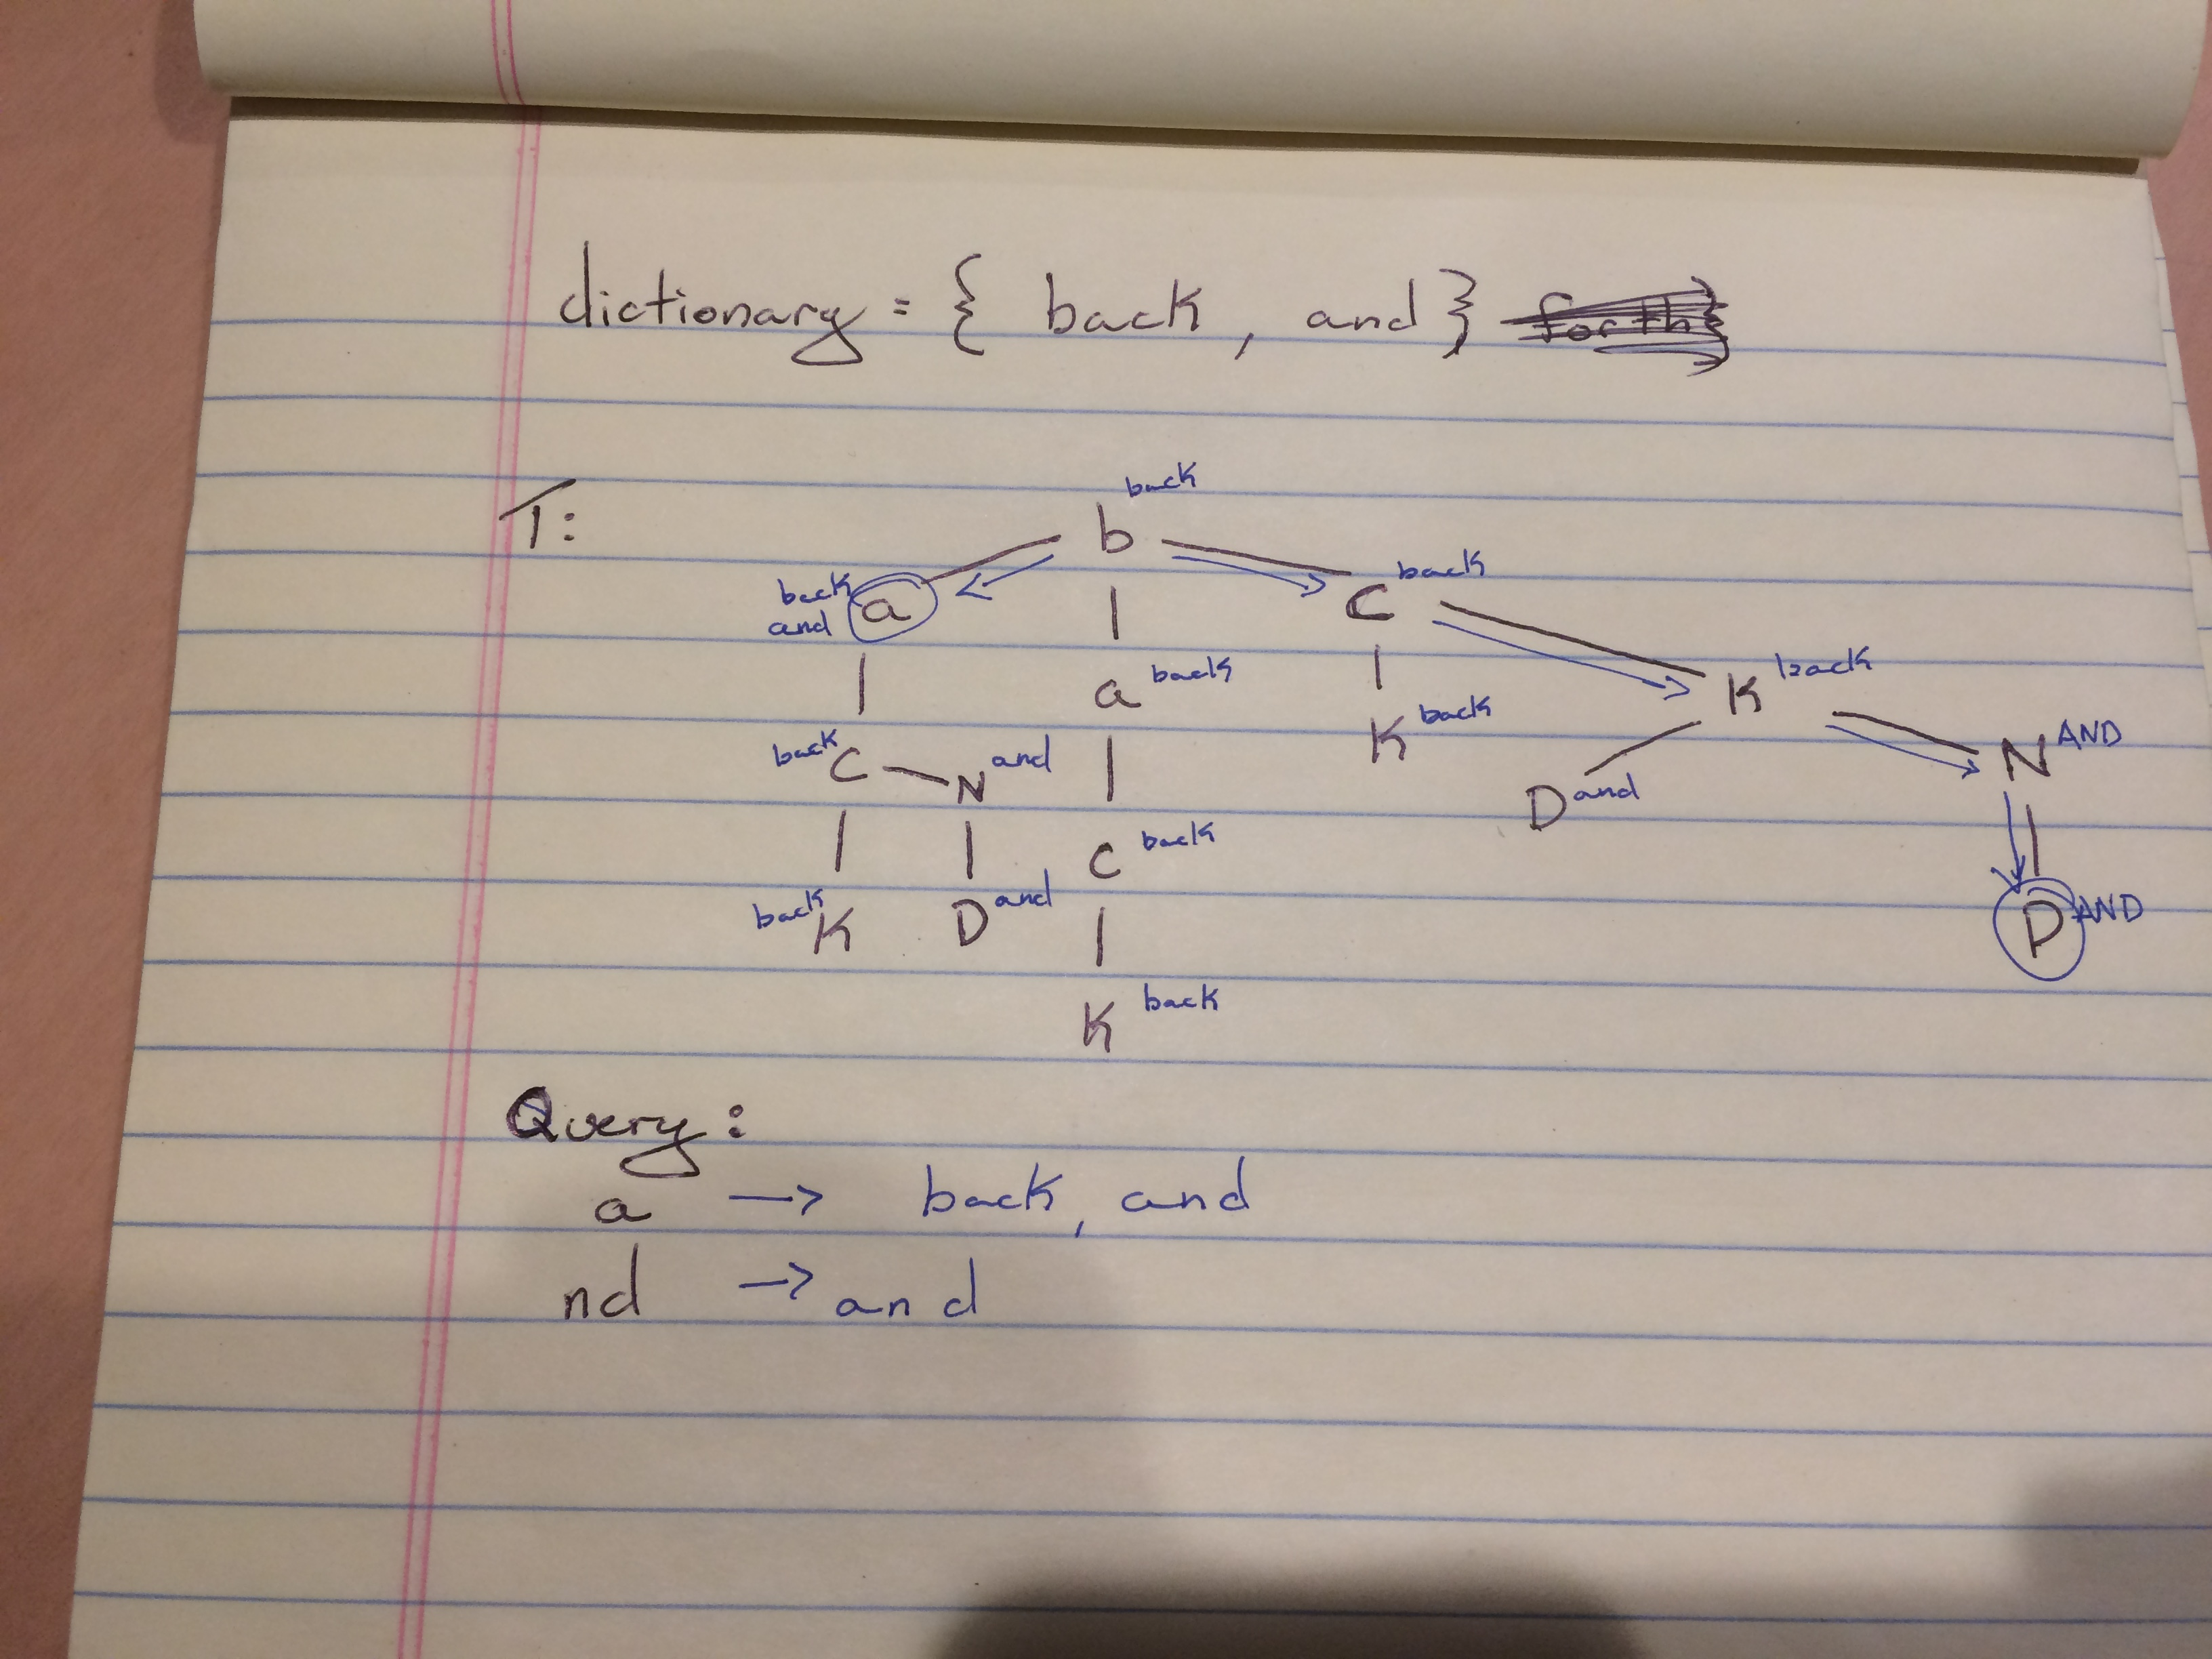
\includegraphics[width=\textwidth]{example2}

%%%%%%% end Problem 2 %%%%%%%%%%%%%%%%%%%%%%%%%%%%%%%%%%%%%%%%%%%%%






%%%%%%% start Problem 3 %%%%%%%%%%%%%%%%%%%%%%%%%%%%%%%%%%%%%%%%%%%
\section{Problem 3}
%%%%%%% Mathematical Formulation %%%%%%%%%%%%%%%%%%%%%%%%%%%%%%%%%%
\subsection{Mathematical Formulation}
Given a network of size $N$ which forms a rooted tree if the sink and all its incident edges are removed, give a worst
case linear time algorithm to determine the maxflow for the set.

%%%%%%% Algorithm %%%%%%%%%%%%%%%%%%%%%%%%%%%%%%%%%%%%%%%%%%%%%%%%%

\subsection{Solution}
Important Confusing Data Structures: (we asume that these are filled out already)
\begin{itemize}
    \item LinkedList[N] \textbf{edgeOut} : stores the indices of the nodes that the
    \item int[N][N] \textbf{cap} : keeps track of capacities between node i and node j
    \item int[N] \textbf{parent} : keeps track of who the parent is for each node i
\end{itemize}

The main functionality of this will be to recursively determine the maximum capacity that each edge has with the
base case being node connected to the sink and the sum of the flow values from the source to the nodes that it
connects to will be the value we return.

\begin{algorithm}[H]
\caption{Main}
\begin{algorithmic}
    \Procedure{control}{}
        \State $flowValue = 0$
        \For{each node $n$ in edgeOut[0]}
            \State flowValue += \Call{calcFlow}{node}
        \EndFor
        \State \Call{print}{flowValue}
    \EndProcedure
    \Procedure{calcFlow}{int node}
        \State value = 0; p = parent[node]
        \If{node is sink}
            \State return cap[p][sink]
        \Else
            \For{node $n\in$ edgeOut[node]}
                \State value += calcFlow(node)
            \EndFor
        \EndIf
        \State return \Call{min}{cap[p][node], value}
    \EndProcedure
\end{algorithmic}
\end{algorithm}


%%%%%%% Correctness %%%%%%%%%%%%%%%%%%%%%%%%%%%%%%%%%%%%%%%%%%%%%%%
\newpage
\subsection{Correctness}
%%%%%%% PROPOSITION 1 %%%%%%%%%%%%%%%
\begin{proposition}
~ \\ \indent This implementation will give us the correct max flow value for a graph which forms
a rooted tree if the sink and all its incident edges are removed
\end{proposition}

\begin{proof}
~ \\ \indent This is due to the properties of the combination of max flow and a rooted tree. With a rooted
tree, each node has 1 parent. This is useful because we then have a basis for the the maximum flow that
can come into the node, then we can calculate the maximum flow that can go out of a node. While doing this
recursively we simply use:
\[ maxFlow(node) =
\begin{cases}
    capacity(inEdge)\ if\ node = sink \\
    minimum
    \begin{cases}
        capacity(inEdge) \\
        \sum_i flow_iFromNode
    \end{cases}
    , else
\end{cases}
\]
Therefore our base case is the sink and we build backwards from there taking the minimum of the capacity
of the edge leading into the node and the sum of the flows of the forward edges.

When we have recursively called this, each of the flowValues going from source to each node it connects to
has the appropriate value of the maximum flow that can be pushed through that node. Therefore summing them
up will give us the maximum flow for the graph
\end{proof}


%%%%%%% Analysis %%%%%%%%%%%%%%%%%%%%%%%%%%%%%%%%%%%%%%%%%%%%%%%%%%
\subsection{Analysis}
For the following analysis, we assume that we have N nodes and at most 2$\cdot$N edges.

%%%%%%% PROPOSITION 1 %%%%%%%%%%%%%%%
\begin{proposition}
\label{numq}
The \underline{time complexity} of this algorithm is \textbf{O(N)}
\end{proposition}

\begin{proof}
This is due to the fact that we will essentially only visit each node 1 time since each node can only have
one parent (due to the tree property) $\implies$ we have a linear algorithm.
\begin{center}
    Giving us a time complexity of \textbf{O(N)}
\end{center}
\end{proof}

%%%%%%% Example %%%%%%%%%%%%%%%%%%%%%%%%%%%%%%%%%%%%%%%%%%%%%%%%%%%

\subsection{An Example}
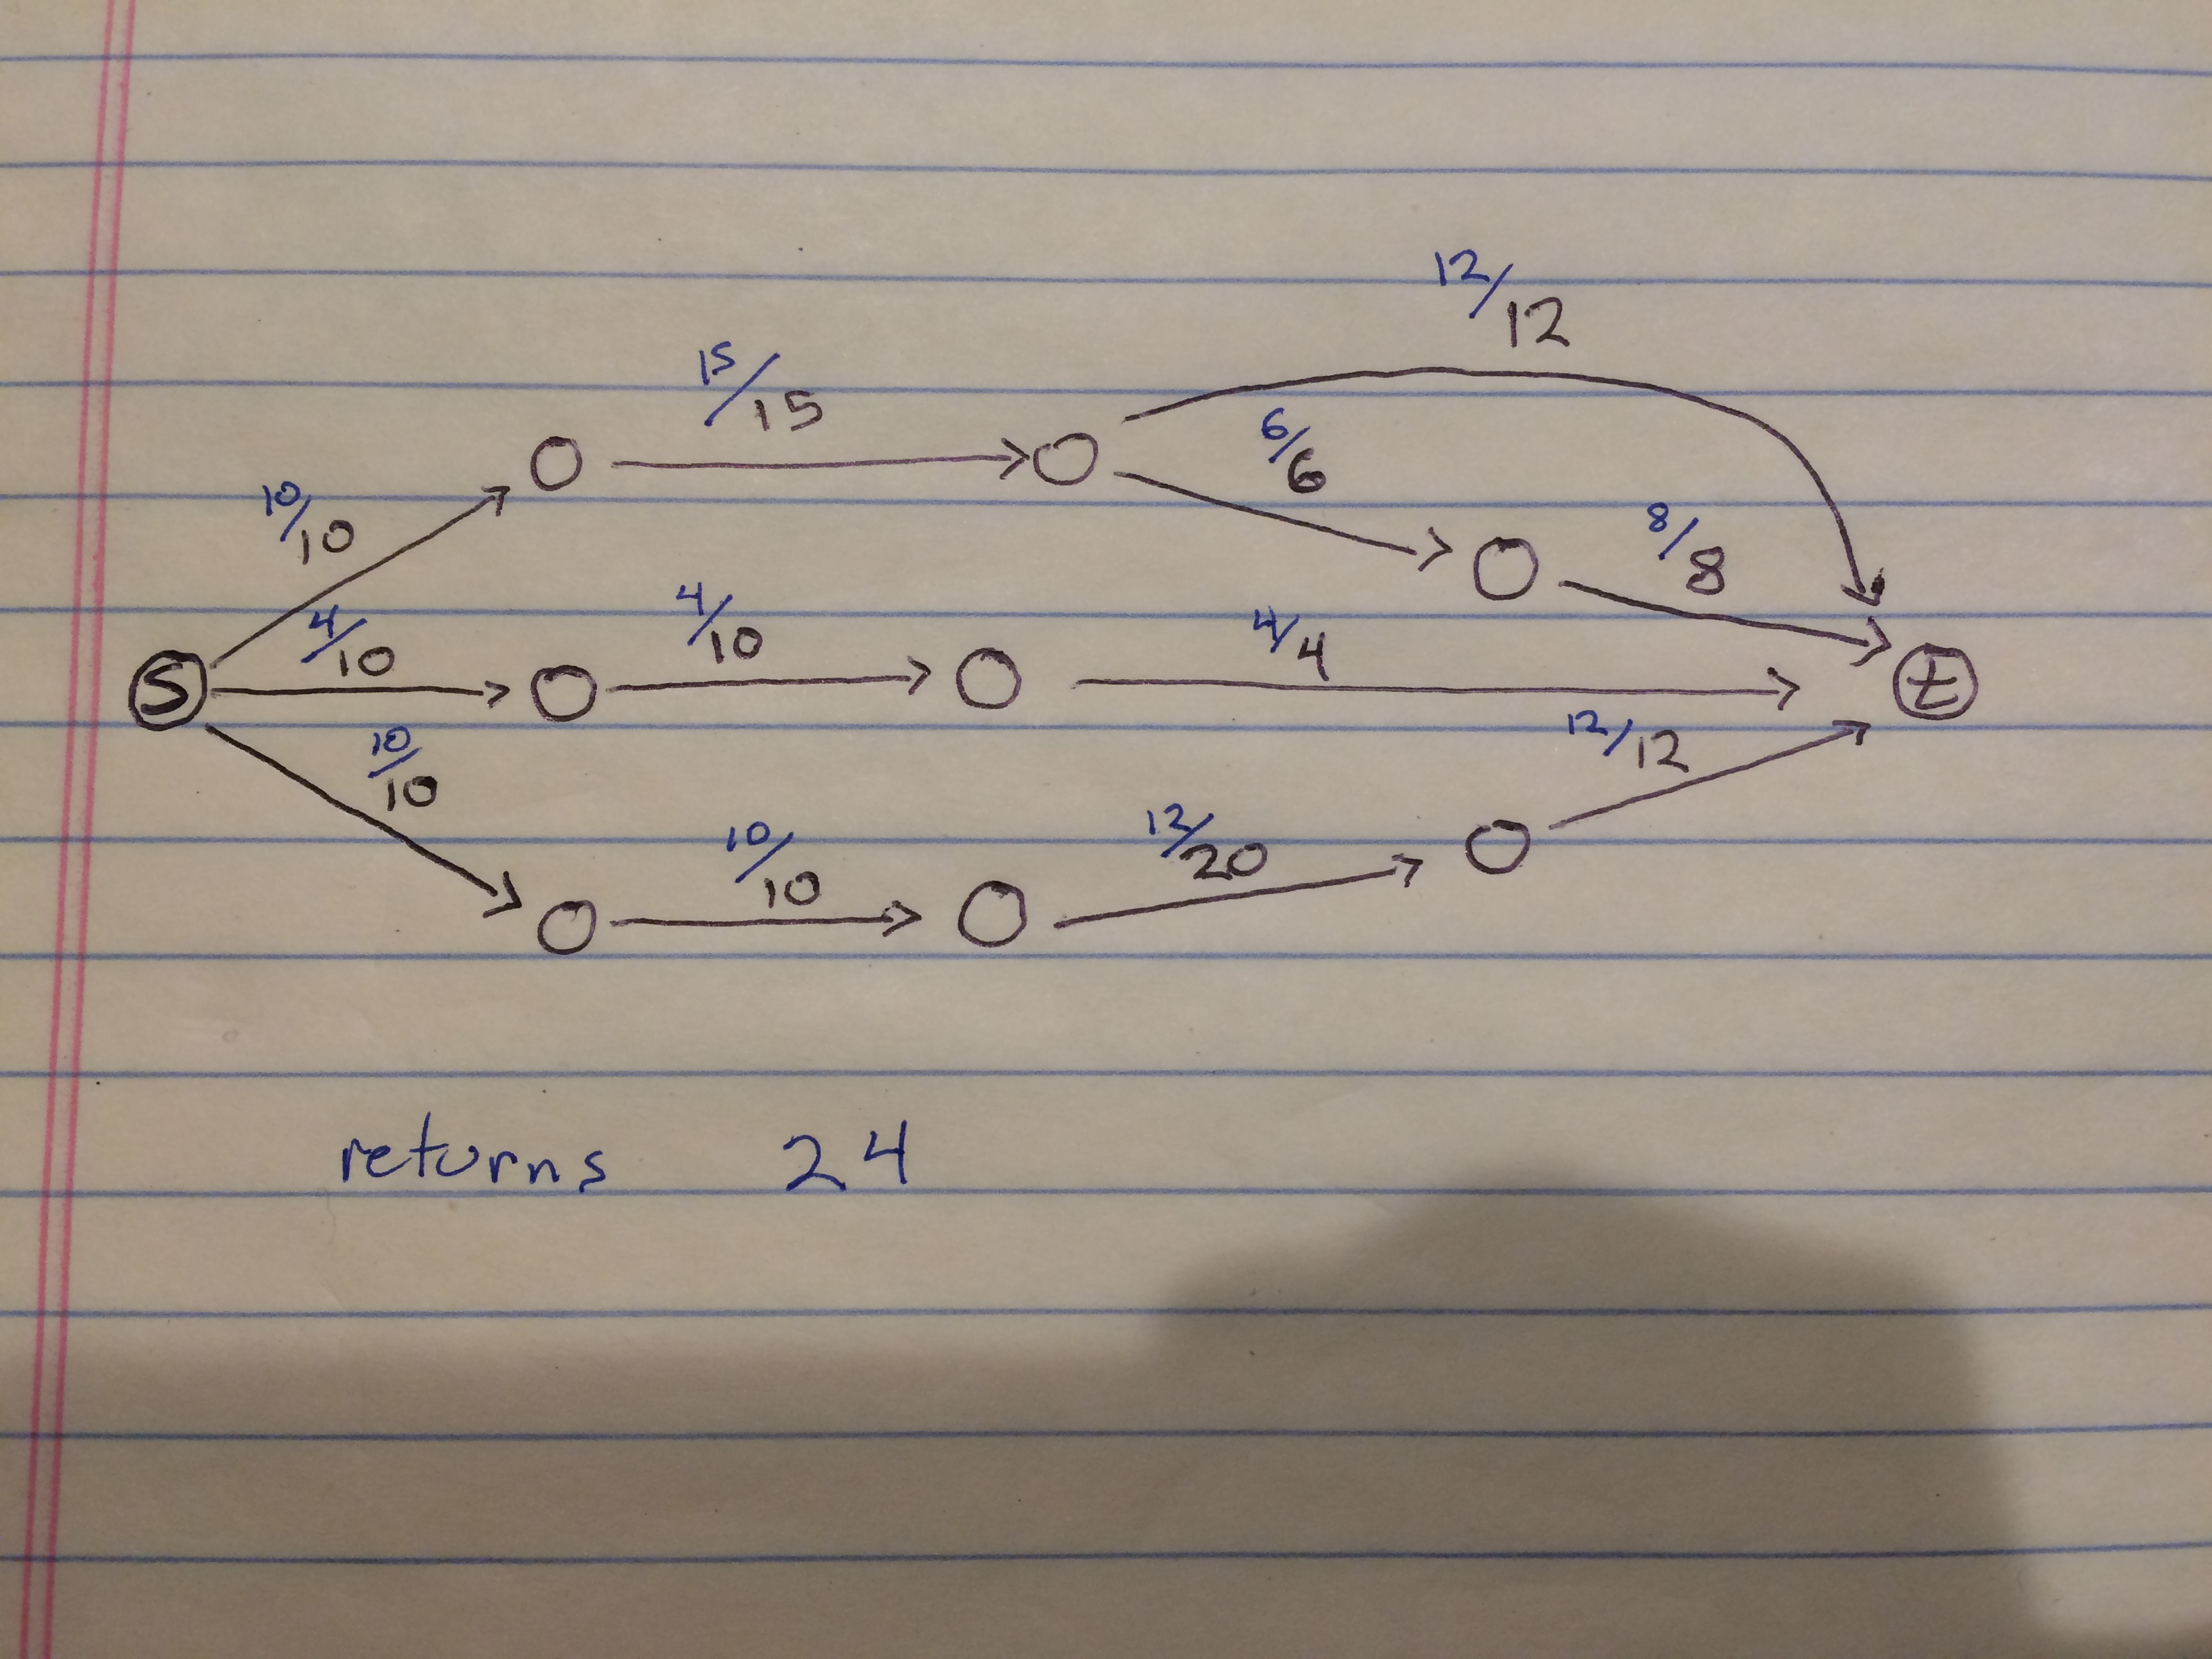
\includegraphics[width=\textwidth]{example3}

%%%%%%% end Problem 3 %%%%%%%%%%%%%%%%%%%%%%%%%%%%%%%%%%%%%%%%%%%%%
\newpage






%%%%%%% start Problem 4 %%%%%%%%%%%%%%%%%%%%%%%%%%%%%%%%%%%%%%%%%%%
\section{Problem 4}
%%%%%%% Mathematical Formulation %%%%%%%%%%%%%%%%%%%%%%%%%%%%%%%%%%
\subsection{Mathematical Formulation}
Given two sets $d_1, d_2$ which are both of size $N$ and are sorted in ascending order, determine, when combined,
what the median number is between the two of them i.e. the $n^{th}$ smallest number.

%%%%%%% Algorithm %%%%%%%%%%%%%%%%%%%%%%%%%%%%%%%%%%%%%%%%%%%%%%%%%

\subsection{Solution}
The main functionality of this algorithm is to perform a form of set reducing keeping with the knowledge that half
of the numbers are smaller and half of the numbers are bigger every time from each sub set recurance happening.
Therefore when we get down to just two numbers we can just pick the smaller. So to start off this algorithm we
would use $System.out.println(calculateMid(d_1, d_2, 0, N-1, 0, N-1))$

\begin{algorithm}[H]
\caption{Main}
\begin{algorithmic}
    \Procedure{calculateMid}{$d_1,d_2,l_1,h_1,l_2,h_2$}
        \State $mid_1 = l_1 + \floor{\frac{h_1 - l_1}{2}}$; $mid_2 = l_2 + \floor{\frac{h_2 - l_2}{2}}$;
        \State $m_1 = d_1[mid_1]$; $m_2 = d_2[mid_2]$;
        \If{$m_1 \textgreater m_2$}
            \If{$l_1 == m_1 \&\& l_2 == m_2$}
                \State return $m_2$
            \EndIf
            \State $h_1 = mid_1, l_2 = mid_2, diff_1 = h_1 - l_1, diff_2 = h_2 - l_2$
            \If{$diff_1 == diff_2$}
                \State return \Call{calculateMid}{$l_1, h_1, l_2, h_2$}
            \ElsIf{$diff_1 \textgreater diff_2$}
                \State return \Call{calculateMid}{$l_1, h_1-1, l_2, h_2$}
            \Else
                \State return \Call{calculateMid}{$l_1, h_1, l_2+1, h_2$}
            \EndIf
        \Else
           \If{$l_1 == h_1 \&\& l_2 == h_2$}
               \State return $m_1$
           \EndIf
           \State $l_1 = mid1, h_2 = mid2, diff_1 = h_1 - l_1, diff_2 = h_2 - l_2$
           \If{$diff_1 == diff_2$}
               \State return \Call{calculateMid}{$l_1, h_1, l_2, h_2$}
           \ElsIf{$diff_1 \textgreater diff_2$}
               \State return \Call{calculateMid}{$l_1+1, h_1, l_2, h_2$}
           \Else
               \State return \Call{calculateMid}{$l_1, h_1, l_2, h_2-1$}
           \EndIf
        \EndIf
    \EndProcedure
\end{algorithmic}
\end{algorithm}


%%%%%%% Correctness %%%%%%%%%%%%%%%%%%%%%%%%%%%%%%%%%%%%%%%%%%%%%%%

\subsection{Correctness}
%%%%%%% PROPOSITION 1 %%%%%%%%%%%%%%%
\begin{proposition}
~ \\ \indent This algorithm will correctly give us the n$^{th}$ lowest number given an input of two distinct
sets $d_i, d_j$ of ordered integers each of length $N$.
\end{proposition}

\begin{proof}
~ \\ \indent Mathematically speaking each time that we perform this algorithm, we are decreasing our search set
size by half or half - 1 depeneding on the initial size i.e. if initial size of the set is N and N/2 is a fraction
and not a whole number, then we will be reducing by N/2 - 1 everytime. Regardless we keep reducing and everytime
we are gauranteed that a quarter of our set is smaller and a quarter of our set is larger than some range.

This is because when we reset our pointers everytime we are doing so with the intention
that if $m_1 \in d_1 \textless m_2 \in d_2$ Then we can be assured that all numbers less than $m_1$
are not our midpoint and all numbers greater than $m_2$ are not are midpoint. Therefore we continue like
this until we are left with only one number in $d_1$ and one number in $d_2$  at which point we know that
there are $N-1$ numbers less than them and $N-1$ numbers greater than them. Therefore choosing the smaller
of the two will give us the $N^{th}$ smallest.
\end{proof}


%%%%%%% Analysis %%%%%%%%%%%%%%%%%%%%%%%%%%%%%%%%%%%%%%%%%%%%%%%%%%
\subsection{Analysis}

%%%%%%% PROPOSITION 1 %%%%%%%%%%%%%%%
\begin{proposition}
\label{numq}
The \underline{time complexity} of this algorithm is \textbf{O(log(N))}
\end{proposition}

\begin{proof}
According to the Masters Theorem since our ruccurence is $T(N) = T(N/2) + 2$, this is a log(N) problem
\begin{center}
    Giving us a time complexity of \textbf{O(log(N))}
\end{center}
\end{proof}

%%%%%%% Example %%%%%%%%%%%%%%%%%%%%%%%%%%%%%%%%%%%%%%%%%%%%%%%%%%%

\subsection{An Example}
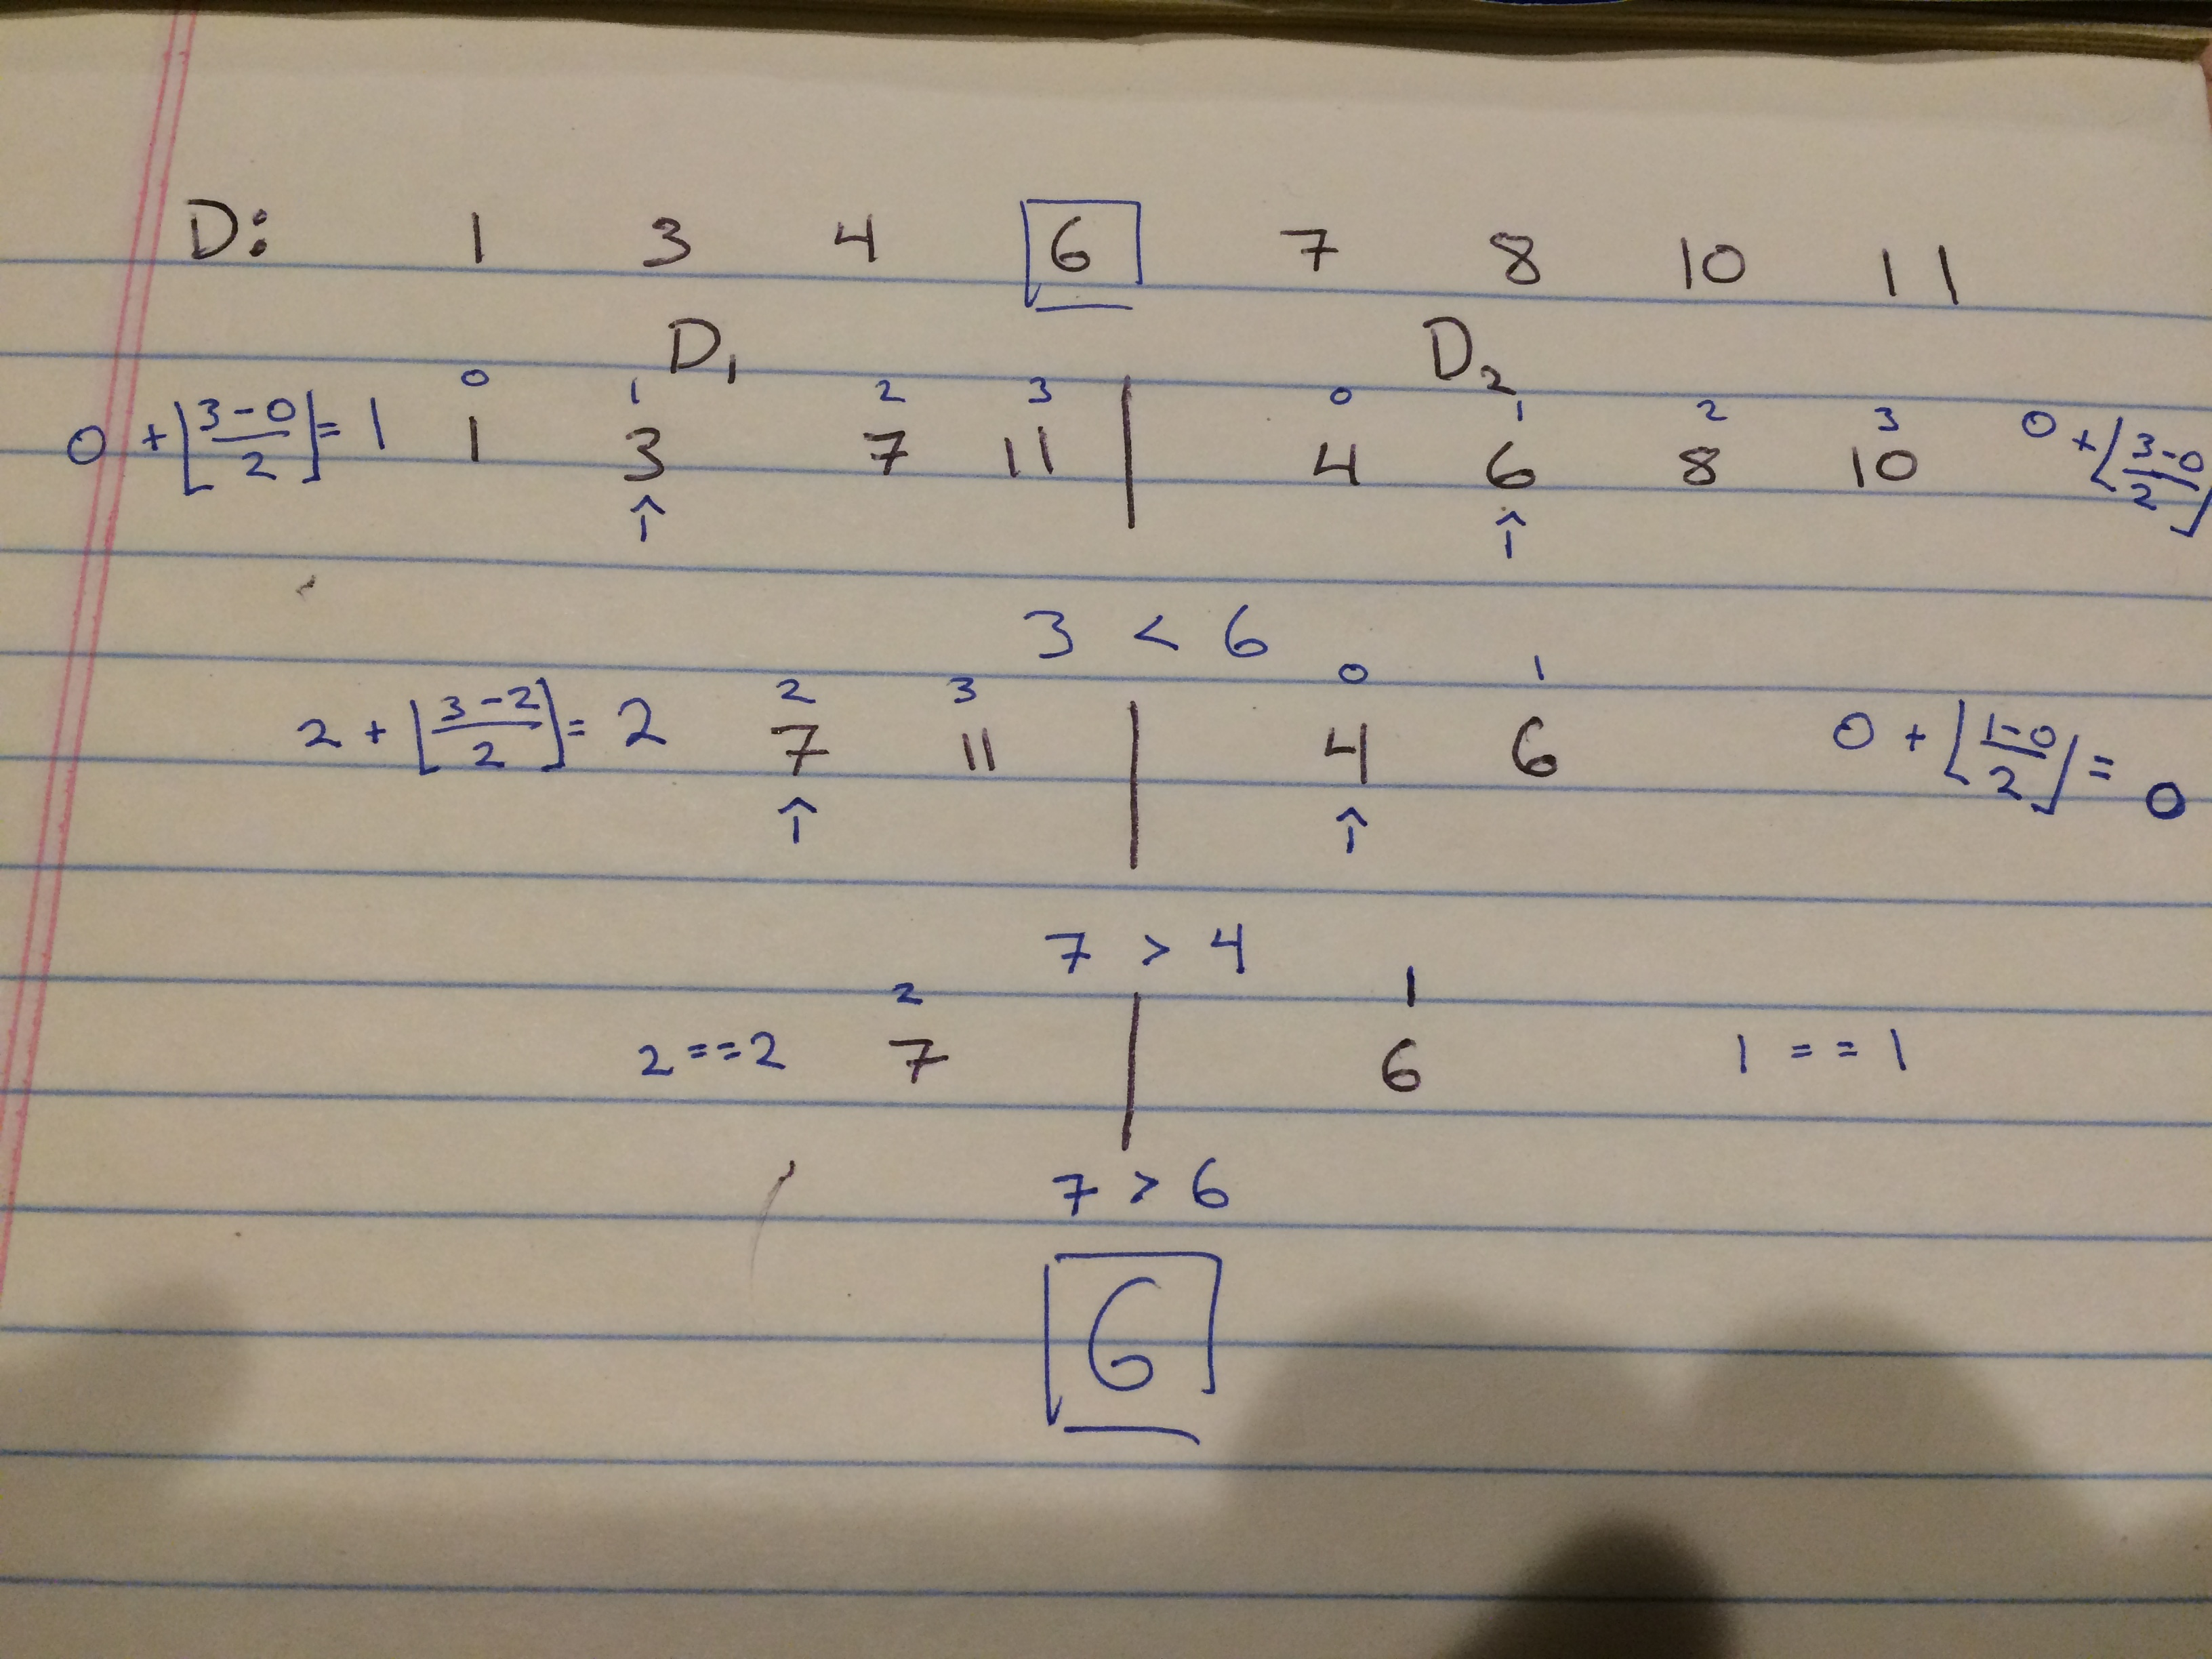
\includegraphics[width=\textwidth]{example4}

%%%%%%% end Problem 4 %%%%%%%%%%%%%%%%%%%%%%%%%%%%%%%%%%%%%%%%%%%%%
\newpage





%%%%%%% start Problem 5 %%%%%%%%%%%%%%%%%%%%%%%%%%%%%%%%%%%%%%%%%%%
\section{Problem 5}
This problem is NP-Complete.

We begin by prooving NP by describing the certificate in polynomial time meaning,
given $k$ sets of jobs, say we have $h$ hours in total, for each job, we check to see that every other job does
not have any overlapping hours. This can be done in $h^2$ time by simply checking for each hour if there exists
another hour in another job that overlaps it.

Next we must proove that I is NP-Hard. We do this by polonomially reducing it from an Independent Set i.e.
let this problem be I, $INDEPENDENT\_SET \leq_P I$. Given a graph, if we can find an independent set of at least
size $k$ then we are gauranteed to be able to find a set of jobs of at least size $k$. We do this by having each
vertex $v \in G$ represent a job $j \in I$ and each edge, $e_{l,k} = v_l - v_k$, represent an overlapping time
interval between jobs $j_l$ and $j_k$. Therefore we can say that $\exists$ a set of nodes $v_i \in G$ which are
an independent set of size $\geq k$ iff $\exists$ a set of jobs $j_i \in I$ which do not overlap of size $\geq k$.


($\Rightarrow$) Given an independent set of at least size $k$ then we know that there are at least $k$ nodes with no
edges between them, therefore if we convert to a set of jobs as described above, there would exist at least $k$
jobs with no overlapping times which solves our problem.

($\Leftarrow$) Given a set of at least $k$ jobs with no overlapping times, then we can see that if each job where
a node and each overlapping time an edge between two of those nodes, that there would be an independent set of
at least size $k$ as well.

Therefore since both NP and NP-Hard, we know that this problem is NP-Complete. $\Box$

%%%%%%% end Problem 5 %%%%%%%%%%%%%%%%%%%%%%%%%%%%%%%%%%%%%%%%%%%%%
\newpage




%%%%%%% start Problem 6 %%%%%%%%%%%%%%%%%%%%%%%%%%%%%%%%%%%%%%%%%%%
\section{Problem 6}
%%%%%%% Mathematical Formulation %%%%%%%%%%%%%%%%%%%%%%%%%%%%%%%%%%
\subsection{Mathematical Formulation}
Given $N$ Districts numbered 1..N ($\{P_1 ... P_N\}$), each of which having $m$ registered voters makine
$N\cdot m$ registered voters in total which each votes for either party A or party B. We will determine wheather
or not it is possible for either party to be GerryMandered

%%%%%%% Algorithm %%%%%%%%%%%%%%%%%%%%%%%%%%%%%%%%%%%%%%%%%%%%%%%%%

\subsection{Solution}
The main functionality of this algorithm is to treat it as a DP problem. The first thing that we do is separate
the sets of A-majority districts and B majority districts keeping track of what the running difference is in
each group. If the difference is equal, then we know that this is not susceptible to gerrymandering (see corallary 7).
Otherwise we choose whichever one has a larger difference as what we should determine to be true.

\begin{algorithm}[H]
\caption{Initialization and Control Method}
\begin{algorithmic}
    \Procedure{Control}{set P}
        \State $A, B \gets$ initialized; sumA, sumB = 0; N = size(P)
        \For{$p_i \in P$}
            \State $diff = p_i.A - p_i.B$
            \If{$diff \geq 0$}
                \State $A.insert(diff)$
                \State sumA += diff
            \Else
                \State diff *= -1
                \State $B.insert(diff)$
                \State sumB += diff
            \EndIf
        \EndFor
        \If{$sumA\ \textgreater\ sumB$}
            \If{size(A) == 1}
                return false;
            \EndIf
            \State return \Call{hasGM}{A, sumA, B, sumB, N}
        \ElsIf{$sumA\ \textless\ sumB$}
            \If{size(B) == 1}
                return false;
            \EndIf
            \State return \Call{hasGM}{B, sumB, A, sumA, N}
        \ElsIf{$sumA == sumB$}
            \State return false;
        \EndIf
    \EndProcedure
\end{algorithmic}
\end{algorithm}

Once we have decided which set is a viable candidate for gerrymandering, W.L.O.G. we can denote this as
$set_1$ which has a majority of value $sum_1$ and the one which is not as $set_2$ with a majority of value
$sum_2$. What we do then is arrange 2 sets of differences for those with $set_1$ as the dominant and another
for those with $set_2$ such that they are organized by number of Districts that comprise them. i.e. level 2
has all combinations of size 2 of districs.  (See proof for more details)

\begin{algorithm}[H]
\caption{Dynamic Programming Solution}
\begin{algorithmic}
    \Procedure{hasGM}{$set_1, sum_1, set_2, sum_2, N$}
        \State LinkedList\textless Integer\textgreater[ ] $S_1 \gets$ \Call{buildDpTable}{$set_1, sum_1, N$}
        \State LinkedList\textless Integer\textgreater[ ] $S_2 \gets$ \Call{buildDpTable}{$set_2, sum_2, N$}
        \State $absoluteDiff \gets sum_1 - sum_2$
        \For{$numElmt_1 \in [S_1.length-1, 0]$}
            \State $numElmt_2 \gets (\frac{N}{2} - numElmt_1) - 1$
            \If{$numElmt_2 == -1$}

            \Else
                \For{int $e_1 \in S_1[numElmt_1]$}
                    \For{int $e_2 \in S_2[numElmt_2]$}
                        \State $diff \gets e_1 - e_2$
                        \If{$(e_1 - e_2 \leq 0)\ ||\ (e_1 - e_2 \geq absoluteDiff)$}
                            \State continue;
                        \EndIf
                        \State return true;
                    \EndFor

                \EndFor
            \EndIf
        \EndFor
        \State return false;
    \EndProcedure
\end{algorithmic}
\end{algorithm}

\begin{algorithm}[H]
\caption{Helpers}
\begin{algorithmic}
    \Procedure{buildDpTable}{$set, size, N$}
        \State $N = minimum(set.size(), N/2)$; height = 0;
        \State $boolean[N][size] dp \gets$ initialized
        \For{district, $d \in set$}
            \For{$row \in [height, -1]$} // decrease
                \If{row == -1}
                    \State dp[0][d] = true;
                \Else
                    \For{$i \in [0, size-1]$}
                        \If{dp[row][i] \&\& (i + d) \textless\ size}
                            \State dp[row+1][i + d] = true;
                        \EndIf
                    \EndFor
                \EndIf
                \If{height $\textless$ N-2}
                    height++
                \EndIf
            \EndFor
        \EndFor
        \State return \Call{getBag}{dp};
    \EndProcedure
    \Procedure{getBag}{boolean[][] $set_{dp}$}
        \State LinkedList\textless Integer \textgreater[$set_{dp}.length$] $bag \gets$ initialized
        \For{$row \in set_{dp}.length$}
            \For{$col \in set_{dp}[row].length$}
                \If{$set_{dp}$}
                    \State bag[row].\Call{insert}{col}
                \EndIf
            \EndFor
        \EndFor
        \State return bag;
    \EndProcedure
\end{algorithmic}
\end{algorithm}

%%%%%%% Correctness %%%%%%%%%%%%%%%%%%%%%%%%%%%%%%%%%%%%%%%%%%%%%%%

\subsection{Correctness}
%%%%%%% COROLLARY 1 %%%%%%%%%%%%%%%%%
\begin{corollary}
~ \\ \indent Given $N$ Precincts = $P$, if we define the total number of voters for party A as \\
$sumA = \sum_{i=1}^{N} (A\ voters\ in\ p_i)$ and likewise the total number of voters for party B as
$sumB = \sum_{i=1}^{N} (B\ voters\ in\ p_i)$ then the difference, $diff = sumA - sumB$. if $diff \leq 0$
then it is impossible for Gerrymandering is impossible.
\end{corollary}

\begin{proof}
~ \\ \indent We will proove by contradiction. Say Gerrymandering is possible for party A, then that implies that we
can have two subsets $P_1'$ and $P_2'$ s.t. $P_1' \cup P_2' = P$ and $P_1' \cap P_2' = \emptyset$ and the sum of
voters for A in $P'1$ ($sumA_1$) $\textgreater$ the sum of voters for B in $P'1$ ($sumB_1$) and same for those in
$P_2'$ ($sumA_2 \textgreater sumB_2$). This would mean then that $sumA_1 - sumB_1 \textgreater 0$ and
$sumA_2 - sumB_2 \textgreater 0$ which means that $(sumA_1 - sumB_1) + (sumA_2 - sumB_2) \textgreater 0$. However
$(sumA_1 - sumB_1) + (sumA_2 - sumB_2) = (sumA_1 + sumA_2) - (sumB_1 + sumB_2) = sumA - sumB \leq 0$ which gives
us a contradiction.
\end{proof}


%%%%%%% PROPOSITION 1 %%%%%%%%%%%%%%%
\begin{proposition}
~ \\ \indent Given two sets of differences that are organized by number of precincts used to create the returned
value $D_A, D_B$ (i.e. $D_A(3)$ contains a list of integers which have been composed using 3 districtcs) and the
total difference between sets 1 and 2 being a positive number $diff_D$, we can determine wheather or not
Gerrymandering is possible.
\end{proposition}

\begin{proof}
~ \\ \indent We first define how $diff_D$ is involved. We know that $diff_D = SUM(A) - SUM(B)$ and this we can
say is $sumA - sumB = (sumA_1 + sumA_2) - (sumB_1 + sumB_2) = (sumA_1 - sumB_1) + (sumA_2 - sumB_2)$ where
$sumA_1$ corresponds to a subset of A-dominant districts and $sumB_1$ corresponds to a subset of A-dominant districts.
Then it follows by Gerrymandering definition that for A to be succeptible, it must win in both sub-groups and the
two subgroups must be of equal size. Therefore we can say that both $(sumA_1 - sumB_1)$ and $(sumA_2 - sumB_2)$
must be positive i.e. $\textgreater 0$.  Since we have the relation then that $(sumA_1 - sumB_1) + (sumA_2 - sumB_2) = diff_D$
$\implies (sumA_1 - sumB_1), (sumA_2 - sumB_2) \textless diff_D$ since neither can be positive.  Therefore it is sufficient
to show that only one of these is within those bounds since it would gaurantee the other to be as well (similar argument
as in Corollary above). So what we do then is to create sets using our given $D_A, D_B$ of set sizes that are equal
to $\frac{N}{2}$ and checking to see each combination if the difference
$e_1 - e_2,\ where\ e_1 \in D_A[i], e_2 \in D_B[\frac{N}{2}-i]$ is within the bounds.  When we have done this we
are gauranteed that the complement set (not important what it is) is also within the bounds $\therefore$
Gerrymandering is possible. If we enumerate every possiblity and nothing is found, then we are guaranteed that one
does not exist since we looked at every possibility.
\end{proof}

%%%%%%% Analysis %%%%%%%%%%%%%%%%%%%%%%%%%%%%%%%%%%%%%%%%%%%%%%%%%%
\subsection{Analysis}

%%%%%%% PROPOSITION 1 %%%%%%%%%%%%%%%
\begin{proposition}
\label{numq}
The \underline{time complexity} of this algorithm is \textbf{O(N$^2\cdot$(N + D))}
\end{proposition}

\begin{proof}
This is because our initial control algorithm take only linear time to build up the two sets O(N),
then we make two boolean tables, each one involving: for each element in the set O(N), for each of the
N rows (worst case) O(N), we fully traverse the row O(D) $\implies$ O(N$^2\cdot$D). Then we create a bag
for each one of the tables which takes linear time in relation to the table O(N$\cdot$D). Once we have
done this, for each row in $bag_1$ O(N) we will compare each vertice O(N) (worst case) with every vertice
in $bag_2$ O(N) (worst case) performing a constant operation each time O(1) $\implies$ O(N$^3$). Therefore
we have (in worst case) run time of O($N + N^2\cdot D + N^3$)
\begin{center}
    Giving us a time complexity of \textbf{O(N$^2\cdot$(N + D))}
\end{center}
\end{proof}

%%%%%%% Example %%%%%%%%%%%%%%%%%%%%%%%%%%%%%%%%%%%%%%%%%%%%%%%%%%%

\subsection{An Example}
The example for this would be terrible. I can come in and discuss it fully if my explanaition was lacking
at all. Please do not hesitate to ask.

%%%%%%% end Problem 6 %%%%%%%%%%%%%%%%%%%%%%%%%%%%%%%%%%%%%%%%%%%%%
%%%%%%% end Solution %%%%%%%%%%%%%%%%%%%%%%%%%%%%%%%%%%%%%%%%%%%%%%

\end{document}